\section{研究方案}
\begin{frame}{技术路线图}
    \centering
    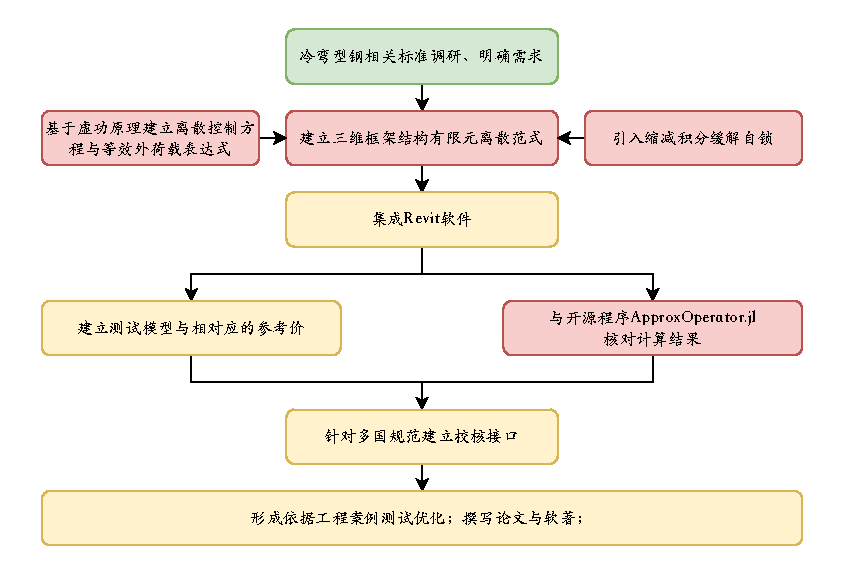
\includegraphics[height=0.9\textheight]{figures/flowchart.pdf}
\end{frame}

\begin{frame}{框架结构有限元范式}
    本项目将采用\textbf{Timoshenko梁假设}的有限元分析方法。

    \vspace{16pt}

{\centering
\begin{tikzpicture}[remember picture]
    \node<1> (week) [anchor=center, yshift=-0pt, xshift=-0pt, align=center] at (0,0) {
        \(\displaystyle \begin{gathered}
            \int_0^L \delta \varepsilon N dx + \int_0^L \delta \kappa M dx + \int_0^L \delta \gamma V dx \\
             = \int_0^L (\delta u \bar{b} + \delta w \bar{q}) dx + (\delta u \bar{N} + \delta w \bar{V} + \delta \phi \bar{M}) \Big|_0^L
        \end{gathered}\)
    };
    \node<2> (week) [anchor=center, yshift=-0pt, xshift=-0pt, align=center] at (0,0) {
        \(\displaystyle \begin{gathered}
            \int_0^L \delta \varepsilon N dx + \int_0^L \delta \kappa M dx + \int_0^L \delta \gamma V dx \\
            = \textcolor{red}{\int_0^L (\delta u \bar{b} + \delta w \bar{q}) dx + (\delta u \bar{N} + \delta w \bar{V} + \delta \phi \bar{M}) \Big|_0^L}
        \end{gathered}\)
    };
    \node<1> (discrete) [align=center] at (0,-2.2) {求解离散控制方程$\displaystyle \boldsymbol K \boldsymbol d = \boldsymbol f$};
    \node<2> (discrete) [align=center] at (0,-2.2) {求解离散控制方程$\displaystyle \boldsymbol K \boldsymbol d = {\color{red}\boldsymbol f}$};
    \node (force) [align=center] at (0,-3.2) {求解等效轴力、弯矩、剪力（$N, M, V$）};
    \node (approximation) [align=center] at (-5.5,2) {节点信息输入\\（$u,v,w,\phi_1,\phi_2,\phi_3$）};
    \node (integration) [align=center] at (0,2) {缩减积分方案};
    \node<1> (boundary) [align=center] at (5.5,2) {等效外荷载与位移边界 \\（$\bar N, \bar M, \bar V, \bar b, \bar q$)};
    \node<2> (boundary) [align=center] at (5.5,2) {\alert{等效外荷载与位移边界} \\ \alert{（$\bar N, \bar M, \bar V, \bar b, \bar q$)}};
    \draw[-{Latex}] (week) -- (discrete);
    \draw[-{Latex}] (approximation) to[bend left] (-2,1);
    \draw[-{Latex}] (integration) -- (week);
    \draw[-{Latex}] (boundary) to[bend right] (2,1);
    \draw[-{Latex}] (discrete) -- (force);
\end{tikzpicture}}
\end{frame}

\begin{frame}{等效外荷载与位移边界}
\begin{columns}[T] % [T] 使三个模块顶部对齐
    \column{0.26\textwidth}
        \begin{block}{永久荷载}
            \small\raggedright
            1. 结构构件自重\\
            2. 土压力\\
            3. 水压力\\
            \textbf{...}
        \end{block}
        
    \column{0.26\textwidth}
        \begin{block}{可变荷载}
            \small\raggedright
            1. 楼面及屋面活荷载\\
            2. 吊车荷载\\
            3. 风荷载\\
            \textbf{...}
        \end{block}
        
    \column{0.26\textwidth}
        \begin{block}{偶然荷载}
            \small\raggedright
            1. 爆炸力\\
            2. 撞击力\\
            \textbf{...}
            \vspace{0.45cm}
        \end{block}
\end{columns}

\vspace{16pt}

\begin{center}
\begin{tikzpicture}[remember picture]
    \node (external) [align=center] at (-5,0) {外荷载};
    \node (residual) [align=center] at (0,0) {等效外荷载  ($\bar N, \bar M, \bar V, \bar b, \bar q$)};
    \node (force) [align=center] at (5,0) {外力向量$f$};
    \draw[-{Latex}] (external) to (residual);
    \draw[-{Latex}] (residual) to (force);
\end{tikzpicture}
\end{center}

\vspace{12pt}

\textit{\footnotesize* 参考《建筑结构荷载规范》GB 50009-2012。}
\end{frame}

\begin{frame}{框架结构有限元范式}
    本项目将采用\textbf{Timoshenko梁假设}的有限元分析方法。

    \vspace{16pt}

{\centering
\begin{tikzpicture}[remember picture]
    \node (week) [anchor=center, yshift=-0pt, xshift=-0pt, align=center] at (0,0) {
         \(\displaystyle \begin{gathered}
            \int_0^L \delta \varepsilon N dx + \int_0^L \delta \kappa M dx + \int_0^L \delta \gamma V dx \\
            = \textcolor{red}{\int_0^L (\delta u \bar{b} + \delta w \bar{q}) dx + (\delta u \bar{N} + \delta w \bar{V} + \delta \phi \bar{M}) \Big|_0^L}
        \end{gathered}\)
    };
    \node (discrete) [align=center] at (0,-2.2) {求解离散控制方程 $\displaystyle \boldsymbol K \boldsymbol d = \textcolor{red}{\boldsymbol f}$};
    \node (force) [align=center] at (0,-3.2) {求解等效轴力、弯矩、剪力（$N, M, V$）};
    \node (approximation) [align=center] at (-5.5,2) {节点信息输入\\（\(u,v,w,\phi_1,\phi_2,\phi_3\)）};
    \node (integration) [align=center] at (0,2) {缩减积分方案};
    \node (boundary) [align=center] at (5.5,2) {\textcolor{red}{等效外荷载与位移边界} \\ \textcolor{red}{（\(\bar N, \bar M, \bar V, \bar b, \bar q\)）}};
    \draw[-{Latex}] (week) -- (discrete);
    \draw[-{Latex}] (approximation) to[bend left] (-2,1);
    \draw[-{Latex}] (integration) -- (week);
    \draw[-{Latex}] (boundary) to[bend right] (2,1);
    \draw[-{Latex}] (discrete) -- (force);
\end{tikzpicture}}
\end{frame}

\begin{frame}{框架结构有限元分析测试与验证}

\begin{columns}[T] % [T] 保证顶部对齐
    \column{0.36\textwidth}
        \begin{block}{理论模型}
            \vspace{-0.2cm} % 去除模块顶部的多余留白
            \centering
            % 核心调整 1：将 node distance 改为 0.8cm，使框与框之间的物理间隙紧凑
            \begin{tikzpicture}[node distance=0.8cm, >=latex]
                % 核心调整 2：minimum height=0.7cm 压低框高；inner ysep=2pt 缩小文字与边框的内边距
                \tikzset{stepnode/.style={align=center, font=\scriptsize\bfseries, text width=3.8cm, minimum height=0.7cm, inner ysep=2pt}}
                
                \node[stepnode] (step1) {1. 依据 Timoshenko 梁理论};
                \node[stepnode, below=of step1] (step2) {2. 推导精确解表达式};
                \node[stepnode, below=of step2] (step3) {3. 校核精确解与数值解的位移};
                
                \draw[->, thick, draw=black!70] (step1) -- (step2);
                \draw[->, thick, draw=black!70] (step2) -- (step3);
            \end{tikzpicture}
            \vspace{0.1cm} 
        \end{block}
        
    \column{0.36\textwidth}
        \begin{block}{开源软件测试}
            \vspace{-0.2cm} % 同上
            \centering
            % 应用完全相同的紧凑参数
            \begin{tikzpicture}[node distance=0.8cm, >=latex]
                \tikzset{stepnode/.style={align=center, font=\scriptsize\bfseries, text width=3.8cm, minimum height=0.7cm, inner ysep=2pt}}
                
                \node[stepnode] (step1) {1. 设计分片实验 (Patch Test)};
                \node[stepnode, below=of step1] (step2) {2. 基于 \texttt{ApproxOperator.jl}\\ 进行数值求解};
                \node[stepnode, below=of step2] (step3) {3. 校核能量误差与\\ 位移误差 (\(L^2, H^1\)误差)};
                
                \draw[->, thick, draw=black!70] (step1) -- (step2);
                \draw[->, thick, draw=black!70] (step2) -- (step3);
            \end{tikzpicture}
        \end{block}
\end{columns}
\vspace{8pt}

\textit{\footnotesize* 商用软件的底层代码未知，无法针对性解耦与二次开发，因此不推荐与商用软件进行比对作为模块的核心验证依据。}

\end{frame}

\begin{frame}{规范校核方案}
% --- 第一行：3 个构件 ---
% 调整列宽：前两个窄一些，第三个宽一些
\begin{columns}[T]
    \column{0.22\textwidth}
        \begin{block}{轴心受拉构件}
            \centering \scriptsize
            \vspace{4pt}
            \(\displaystyle \frac{\textcolor{red}{N}}{A_n} \le f\)
            \vspace{4pt} % 手动撑开高度，与其他长块平齐
        \end{block}
        
    \column{0.26\textwidth}
        \begin{block}{轴心受压构件}
            \centering \scriptsize
            \vspace{4pt}
            \(\displaystyle \frac{\textcolor{red}{N}}{A_{en}} \le f, \quad \frac{\textcolor{red}{N}}{\varphi A_e} \le f\)
            \vspace{4pt} % 手动撑开高度
        \end{block}
        
    \column{0.42\textwidth}
        \begin{block}{受弯构件}
            \centering \scriptsize
            \vspace{4pt}
            \(\displaystyle \frac{\textcolor{red}{M}}{W_{enx}} \le f, \ \frac{\textcolor{red}{V}S}{It} \le f_v, \ \frac{\textcolor{red}{M}}{\varphi_{bx} W_{ex}} \le f\)
            \vspace{4pt}
        \end{block}
\end{columns}

\vspace{6pt}

% --- 第二行：3 个构件 ---
\begin{columns}[T]
    \column{0.22\textwidth}
        \begin{block}{拉弯构件}
            \centering \scriptsize
            \vspace{4pt}
            \(\displaystyle \frac{\textcolor{red}{N}}{A_n} \pm \frac{\textcolor{red}{M_x}}{W_{nx}} \pm \frac{\textcolor{red}{M_y}}{W_{ny}} \le f\)
            \vspace{1.2cm} 
        \end{block}
        
    \column{0.26\textwidth}
        \begin{block}{压弯构件}
            \centering \scriptsize
            \vspace{2pt}
            \(\displaystyle \begin{aligned} \frac{\textcolor{red}{N}}{A_{en}} + \frac{\textcolor{red}{M_x}}{W_{enx}} + \frac{\textcolor{red}{M_y}}{W_{eny}} &\le f \\[0.6em] \frac{\textcolor{red}{N}}{\varphi A_e} + \frac{\beta_m \textcolor{red}{M_x}}{(1 - \frac{N}{N_E'}\varphi) W_{ex}} &\le f \end{aligned}\)
            \vspace{4pt}
        \end{block}
        
    \column{0.42\textwidth}
        \begin{exampleblock}{构件中的受压板件}
            \centering \scriptsize
            \vspace{2pt}
            \(\displaystyle 
            \begin{cases}
            \frac{b_c}{t}, & b/t \le 18\alpha\rho \\[0.4em]
            \left(\sqrt{\frac{21.8\alpha\rho}{b/t}} - 0.1\right)\frac{b_c}{t}, & 18\alpha\rho < b/t < 38\alpha\rho \\[0.4em]
            \frac{25\alpha\rho}{b/t} \cdot \frac{b_c}{t}, & b/t \ge 38\alpha\rho
            \end{cases}\)
            \vspace{8pt}
        \end{exampleblock}
\end{columns}

\vspace{6pt}
\textit{\footnotesize*参考《冷弯薄壁型钢结构技术规范》GB50018-2002。 }
\end{frame}